% Higgs simulation and experiementation section

%  should also include WW ?  yes!

\subsection{Comparison of the ILC Higgs capability with 
HL-LHC projections}

It is appropriate to compare the capabilities of the ILC for precision
Higgs measurement to those of the HL-LHC.  Since the ILC is planned as
an expensive new accelerator project, it should be justified on the
basis that it will qualitatively advance our knowledge of the Higgs
boson over what is possible from the LHC in its high luminosity stage.  
This section will present several such comparisons.

The goal of the ILC is not simply to achieve a high degree of
precision in the measurement of Higgs boson couplings; it is to
discover deviations of the Higgs boson couplings from their Standard
Model predictions and to demonstrate those deviations with a high
degree of confidence.  The strengths of the ILC program are the
 following:
\begin{enumerate}
\item The ILC will report the properties of the Higgs boson in a
  highly model-independent framework.   Our estimate for the ILC capabilities
  are based on an effective field theory (EFT) model that includes
 {\underline{all}}\ dimension-6 operators that appear in the relevant physics
  cross sections at the tree level  (16 operators in all).   Our model
  also includes 2 further parameters to account for possible invisible
  and exotic Higgs decays.  The errors in this model due to
  unaccounted terms are percent-level corrections relative to the new
  physics effects already included in the model.   The analysis includes a
  high-precision determination of the Higgs boson total width. 
 Thus, the ILC will be able to measure  the full array of Higgs 
boson decays and to detect and quantify anomalies in any aspect of this behavior.
\item  For the Higgs boson couplings to $ZZ$, $WW$, and $b\bar b$, 
the ILC will achieve 1\% precision in its initial 250 GeV
  stage.   This is the
 level deemed necessary to be sensitive to the typical predictions 
of the effects of new physics models on the Higgs boson couplings.
\item  If  anomalies are  discovered in the ILC 
250 GeV program, these
  anomalies can be confirmed with an independent data set by
  increasing the energy of the ILC to 500 GeV.   This second energy
  stage will improve the precision of the ILC 
determinations by about a factor of 2.  
\item The ILC, with Higgs bosons tagged by recoil against a $Z$ boson
  and with no trigger requirements, will be able to observe directly
  all manner of exotic Higgs boson decays that might be produced by
Higgs couplings  to  light, weakly coupled  particles.
\end{enumerate}
All of these features go qualitatively beyond what is possible at the 
LHC, or at any hadron collider.

Beyond these conceptual improvements, we can compare the ILC
capabilities quantitatively to the projections released in the HL-LHC
Yellow Report \cite{YR}.   This comparison is given in
Table~\ref{tab:ILCLHC}.   It is not so straightforward to give a
direct apples-to-apples comparison to the estimates presented in the
Yellow Report.    The HL-LHC projections are reported in two
scenarios.  Scenario 1 (S1) is a projection based on our current
understanding of Higgs boson analyses, adding the increased data
available from the HL-LHC.   Scenario 2 (S2) assumes that the current
analyses can be improved by dividing the current theoretical
systematic errors by 2 and dividing the current experimental
systematic errors by $\sqrt{N}$, a factor of 6.   The latter
assumption, in particular, leads to very significant reductions in the
uncertainties.   S2 is intended to model the progress that the LHC
experiments have made in improving their understanding through actual
experience working with the data.  Still, ``past performance is not a 
guarantee of  future results''.

In spirit of the HL-LHC projections, we present multiple estimates of the ILC
capabilities at 250 GeV  in Table~\ref{tab:ILCLHC}.   We consider
these in turn.   The analysis labelled S1* in the table is based
on the highly model-independent framework described in item 1 above.
It is based on 2 ab$^{-1}$ of ILC data at 250~GeV on the reaction
$\ee\to hZ$.   To fix certain EFT operator coefficients, it also makes
use of data on $\ee \to W^+W^-$ at 250~GeV, as well as precision
electroweak measurements.   The analysis also includes
information from LHC that should be available from the 
HL-LHC results.  The LHC measurement of the ratio of the $\gamma\gamma$ and 
$ZZ^*$ branching ratios, which should be almost free of systematic
errors from the Higgs production process, plays an important role, and
the LHC measurments of the 
$\mu^+\mu^-$ and $Z\gamma$ branching ratios are used to constrain
those modes. 
The estimates of measurement errors
for the various ILC observables  are obtained as the result of  full
simulation studies using the ILD and SiD detector models.   The table
of input measurements is 
presented in some detail in Appendix A of \cite{Barklow:2017suo}. 

The LHC S1 estimates do not assume such a model-independent framework.
Among the many model-dependent assumptions in the LHC  analyses, two are
particularly important. They  assume  that the Higgs boson has no decay
modes beyond those predicted in the SM, and they  assume that the Higgs
boson couplings to $WW$ and $ZZ$ are modified only by a rescaling.  In
the ILC EFT analysis, each of these these couplings depends on two
independent constants, called $\eta_{W,Z}$ and $\zeta_{W,Z}$ in
\cite{Barklow:2017suo}.   We can redo the ILC EFT analysis
adding these two assumptions, that is, assuming no
Beyond-Standard-Model decays and assuming $\zeta_{W} = \zeta_Z = 0$.
This gives the uncertainty estimates listed for ILC  in the column S1
in Table~\ref{tab:ILCLHC}.   We consider the comparison of the S1
uncertainties the most direct comparison of the capabilities of  LHC
alone with results of adding the ILC dataset. 
  We emphasize that the S1 analysis is 
simply a recast of the S1* estimates; the ILC inputs are based just 
as firmly in our full-simulation results.

%%%%%%%%%%%%%%%%%%%%%%%%%%%%%%%%%%%%%%%%%%%%5
\begin{table}
\begin{center}
\begin{tabular}{lccccc}
   coupling     &  current  &    S1*     &     S1     &    S2*   &   S2   \\ \hline 
$hZZ$ - LHC  &     11.      &        &       2.5   &        &  1.7 \\ 
\phantom{$hZZ$} - ILC 250 &      &   0.68  &  0.46   &   0.59   &  0.33 \\ 
\phantom{$hZZ$} - ILC 500&      &   0.35  &  0.20  &  -   &  - \\ 
 \hline 
$hWW$ - LHC  &    15.       &        &    3.0     &        &  2.1 \\ 
\phantom{$hWW$} - ILC 250 &      &   0.67 &  0.44   &   0.57   &  0.32 \\ 
 \phantom{$hWW$} - ILC 500 &      &   0.34 &  0.19   &  -   &  - \\ 
   \hline 
$hbb$ - LHC  &    29.       &        &          5.5   &        & 4.0 \\ 
\phantom{$hbb$} - ILC 250 &      &  1.1  & 0.83   &   0.77   &  0.56 \\ 
\phantom{$hbb$} - ILC 500 &      &  0.58  & 0.56   &  -  &  - \\ 
 \hline 
$h\tau\tau$ - LHC  &    17.       &        &              3.6  &        & 2.8 \\ 
\phantom{$h\tau\tau$} - ILC 250 &      &  1.2  &  0.98   &   0.90   &  0.70 \\ 
\phantom{$h\tau\tau$} - ILC 500 &      &  0.74  &  0.42   &  -   & - \\ 
    \hline 
$hgg$ - LHC  &     15.      &        &            4.0   &        &
                2.8   \\ 
\phantom{$hgg$} - ILC 250 &      &  1.7  &  1.6   &   0.92   &  0.75 \\ 
 \phantom{$hgg$} - ILC 500 &      &  0.95  &  0.91   &   -   & - \\ 
\hline 
$hcc$ - LHC  &    -       &        &           -  &        &  - \\ 
\phantom{$hcc$} - ILC 250 &      &   1.9  &  1.8   &   1.2  &  1.0 \\ 
\phantom{$hcc$} - ILC 500 &      &  1.2  &  1.1   &   -  &  - \\ 
    \hline 
$h\gamma\gamma$ - LHC  &    15.       &        &         3.6  &        & 2.8 \\ 
\phantom{$h\gamma\gamma$} - ILC 250  &      &   1.2  &  1.1  &   1.2   &  1.0\\ 
 \phantom{$h\gamma\gamma$} - ILC 500  &      &   1.0  &  0.97 &   -   &  -\\ 
\hline 
$h\mu\mu$ - LHC  &   70.        &        &     7.6  &        & 7.0 \\ 
\phantom{$h\mu\mu$} - ILC 250 &      &  5.6  &  5.6  &  5.4  &  5.3 \\ 
\phantom{$h\mu\mu$} - ILC 500 &      &  5.1  &  5.0  &  -  &  - \\ 
     \hline 
$htt$ - LHC  &   14.        &        &           5.5   &        &  3.6
  \\  
 \phantom{$htt$} - ILC 500  &        &    6.3    &     6.3      &     -   & -
\\ 
\hline \hline
$\Gamma_{tot}$ - ILC 250 &  &   2.5   &   1.4       &    1.6          &   0.82  \\ 
\phantom{$\Gamma_{tot}$} - ILC 500 & & 1.6 &  0.69 & -  & - \\  \hline
\end{tabular}
\end{center}
\caption{ \label{tab:ILCLHC}   Projected uncertainties in the Higgs
  boson couplings for LHC and for   and for ILC at 250~GeV, with
  precision LHC input, in various scenarios.   All values
  are given in percent (\%). The values labeled ``current'' are taken
  from Table 8 of the CMS publication \cite{Sirunyan:2018koj}.   The LHC S1 and
  S2 values are taken from \cite{YR}. The ILC scenarios are as
  described in this paper.  We also include our S1* and S1 projections
including the full ILC data set  with running at 250~GeV and 500~GeV.   The
  bottom lines give, for reference, the projected uncertainties in the
  Higgs boson total width.   We believe that the comparison of the S1
  values  gives the sharpest comparison between the capabilities of LHC
  alone and the capabilities after adding the ILC measurements. }
\end{table}

We have also attempted to produce a set of S2 estimates for the ILC.
These, by construction, go beyond our current understanding.  But it
has been true for electron colliders, just as for hadron colliders,
that actual experience in operating the experiments and working with
the 
data has led  to results that have exceeded the design levels of
performance.  To estimate the possible improvement, 
we have looked for elements in our work that 
are conservatively estimated and for which more detailed effort
making use of actual experience could produce a substantial
improvement.  Most of the improvement factors that we incorporate here
have already been estimated in 
preliminary ILD and SiD analyses.   There is also 
headroom in the ILC design for a possible
increase in luminosity (for example, by improving the tolerances in
the damping rings), but this is not included in our estimates.
  Using the more 
optimistic values as inputs to our 
model-independent analysis, we find the
uncertainties in the column S2*.  Applying also the model-dependent
assumptions
 listed above, we find the uncertainties shown in
 the column S2. 

%%%%%%%%%%%%%%%%
\begin{figure}
\begin{center}
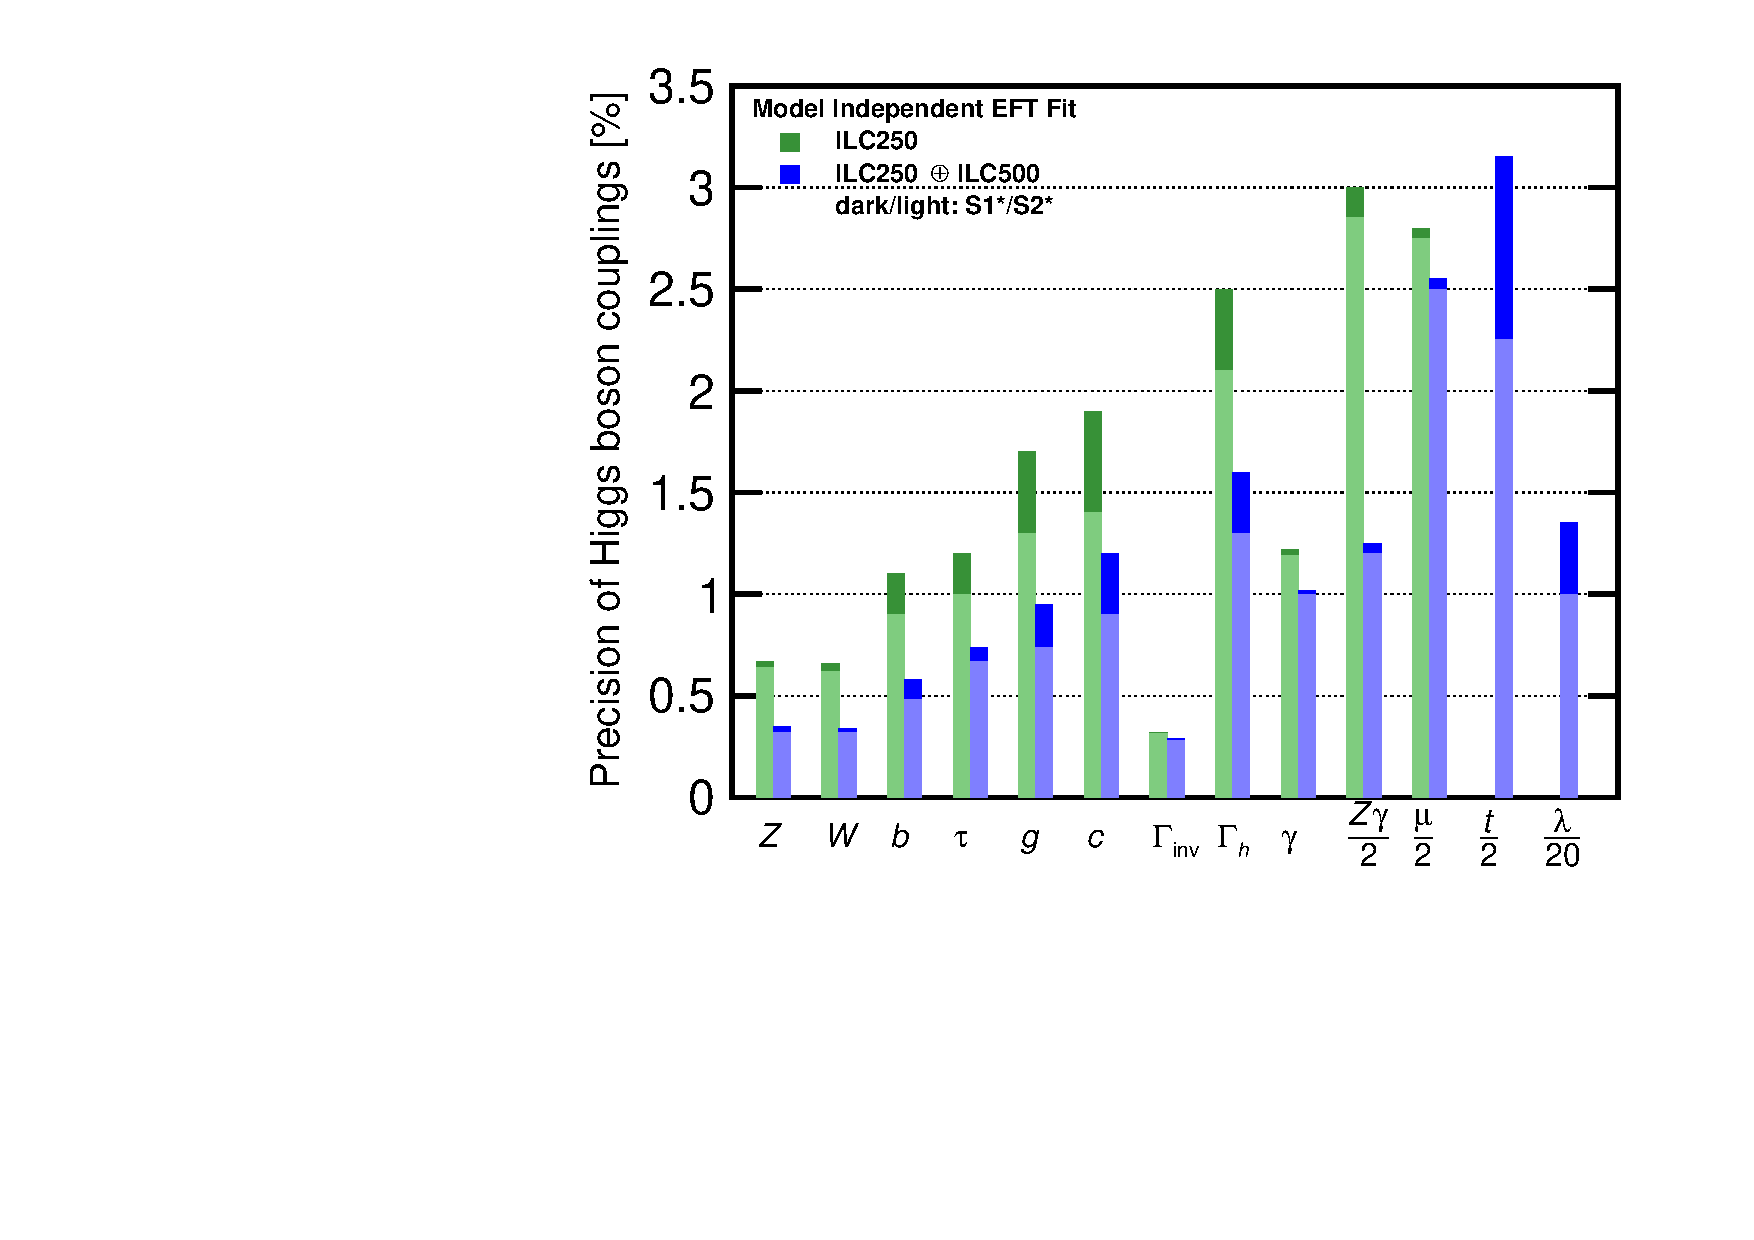
\includegraphics[width=0.85\hsize]{chapters/figures/ModelindepSummary.pdf}
\caption{Projected Higgs boson coupling uncertainties for the ILC
  program at 250~GeV and an energy upgrade to 500~GeV, using the
  highly model-independent analysis presented in \cite{Fujii:2017vwa}. This
  analysis makes use of  data on $\ee\to W^+W^-$ in addition to Higgs
  boson observables and also incorporates projected LHC results, as described
  in the text.  These
values correspond to the  scenario S1* in Table~\ref{tab:ILCLHC}.}
\label{fig:ILCmodelindep}
\end{center}
\end{figure}
%%%%%%%%%%%%%%%%%%%%%%%%%%%%%%%%%%%%%%%%%%%%%%%%%%%%%%%%%%%%%%
%%%%%%%%%%%%%%%%
\begin{figure}
\begin{center}
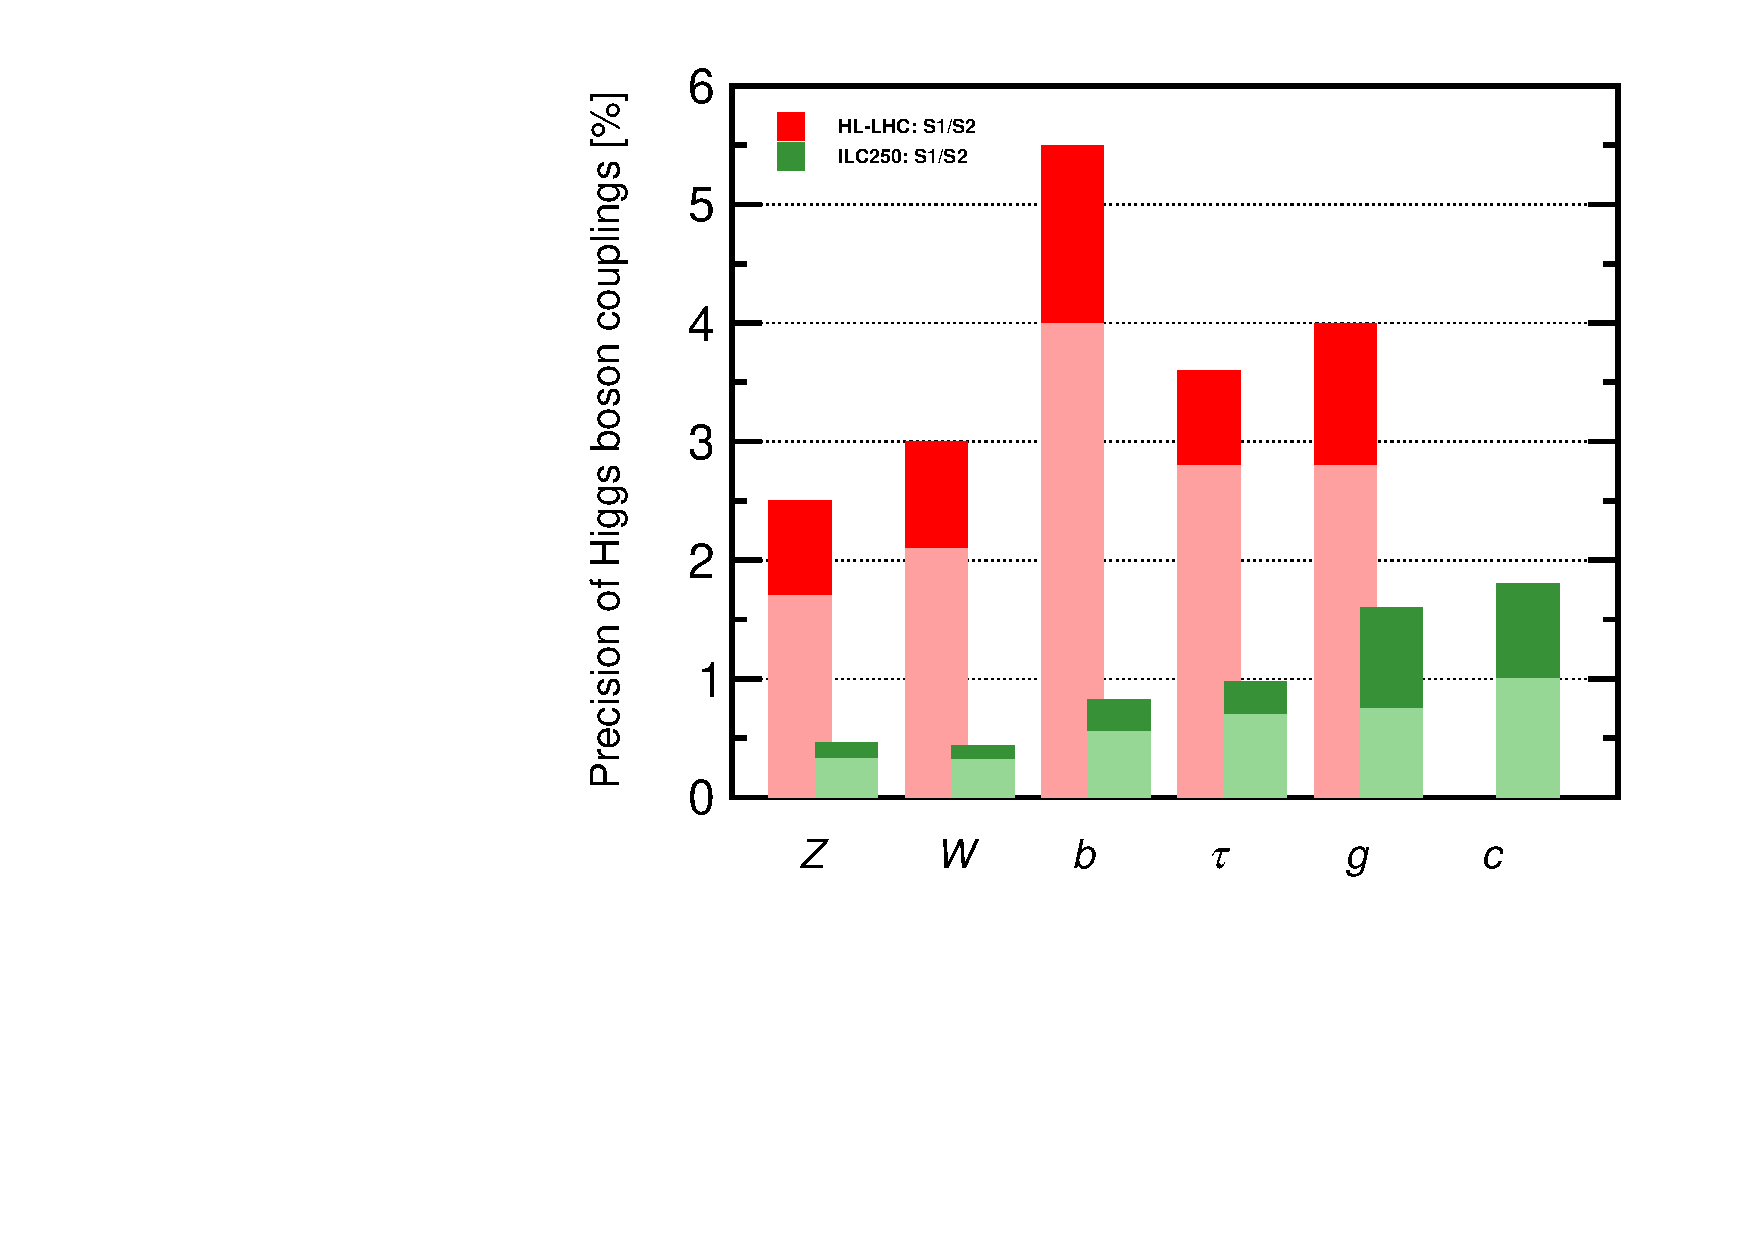
\includegraphics[width=0.85\hsize]{chapters/figures/ModeldepSummary.pdf}
\caption{Projected Higgs boson coupling uncertainties for the LHC and
  ILC
using the model-dependent assumptions appropriate to the LHC Higgs
coupling fit.   The
dark and light red bars represent the projections in the scenarios S1
and S2 presented in  \cite{YR}.    The dark and light green bars represent the
projections in the ILC scenarios S1 and S2 described in the
text.  The dark and light blue bars show the projections for scenarios S1 and S2
when
data from the 500~GeV run of the ILC is included.}
 \label{fig:ILCLHC}
\end{center}
\end{figure}
%%%%%%%%%%%%%%%%%%%%%%%%%%%%%%%%%%%%%%%%%%%%%%%%%%%%%%%%%%%%%%


Figures~\ref{fig:ILCmodelindep} and \ref{fig:ILCLHC}  illustrate the
capabilities of the ILC and the comparison of the ILC and LHC
projections.  Figure~\ref{fig:ILCmodelindep} shows the uncertainty
projections for the 250~GeV stage of the ILC, in the highly
model-independent framework S1*.  In the figure, these results are
compared to results obtained in the same framework with the addition
of data from an energy upgrade to 500~GeV.   This justifies the
statement made above that deviations from the SM seen at the 250~GeV
stage of the ILC can be confirmed with an independent data set after
the upgrade to higher energy.   Figure~\ref{fig:ILCLHC} shows the
comparison of the ILC projections in the S1 and S2 scenarios to the 
projections given for the S1 and S2 HL-LHC scenarios given in
\cite{YR}.  
Note that, while the improvement from the S1 to S2 scenarios is a
matter of conjecture, the improvement from the 250~GeV to the 500~GeV
values is based on completed full-simulation studies.
